\section{Semaine 04 (07/10-11/10) }

\e{Notions abordées :}
\begin{itemize}
	\item Mécanique de MPSI (forces centrales et dynamique du solide).
	\item Dynamique en référentiel non galiléen.
\end{itemize}

\subsection{Exercice 1 : Pendule pesant dans une voiture accélérée}

Une tige homogène de longueur $l$ et de masse totale $m$ est accrochée en un point $A$ du plafond d'une voiture. La voiture est en translation rectiligne d'accélération $a$ par rapport au référentiel terrestre supposé galiléen. 

Le moment d'inertie de la tige par rapport au point $A$ est $J = \frac{1}{3}m l ^2$. On admet que le point d'application de la force d'inertie d'entraînement est le centre d'inertie de la tige.

\begin{enumerate}
	\item Déterminer l'angle d'équilibre du pendule dans le référentiel de la voiture.
	\item Déterminer la période $T$ des petites oscillations du pendule autour de la position d'équilibre.
\end{enumerate}

\subsection{Exercice 2 : Limite de Roche}

\begin{minipage}[c]{\linewidth/2}
	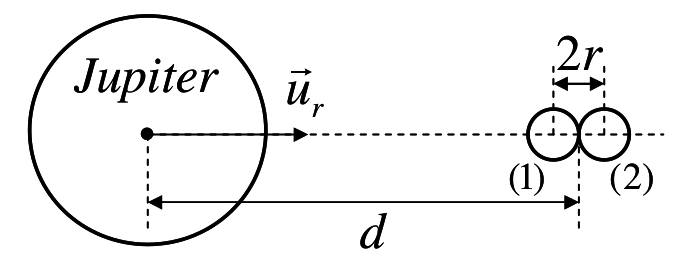
\includegraphics[width=\linewidth]{Images/mp_s04_ex02.png}
\end{minipage}%
\begin{minipage}[c]{\linewidth/2}
	On cherche à déterminer la distance en dessous de laquelle une comète s'approchant de Jupiter se sépare en plusieurs morceaux sous l'effet des forces de marée dues à Jupiter.
	
	On modélise la comète par deux sphères identiques de masses $m$ et de rayon $r$, alignées comme sur le dessin. On suppose que la comète est en orbite circulaire de rayon $d$ autour de Jupiter.
\end{minipage} 

\begin{enumerate}
	\item Montrer que le mouvement du centre d'inertie de la comète est uniforme. Quelle est la nature du mouvement du référentiel barycentrique de la comète par rapport au référentiel de Jupiter ?
	\item Soit $\vec{R}$ la réaction de la sphère $(1)$ sur la sphère $(2)$. Dans le référentiel de la comète, appliquer le PFD à une des deux sphères.
	\item À quelle condition le contact entre les sphères est-il rompu ? Déterminer, sachant que $r \ll d$, la distance limite $d_{lim}$ en dessous de laquelle il ne peut exister de comètes.
\end{enumerate}

\e{Données :} $M_J = \SI{1.9e27}{kg}$, $R_J = \SI{7.1e4}{km}$ et masse volumique de la comète $\rho_c = \SI{1.0e3}{\kilogram\per\cubic\metre}$.

\e{Réponse :} $d_{lim} = \SI{1.8e5}{km}$.

\subsection{Exercice 3 : Usure d'une ligne de TGV}

Un train grande vitesse se dirige vers le sud, depuis Paris (latitude $48.8$°). On considère son mouvement dans le référentiel terrestre non galiléen. Montrer qu'apparaît une réaction horizontale de la voie sur le train. La comparer à la réaction verticale. 



